\section[WireGuard ]{\texorpdfstring{WireGuard
\footnote{\label{fn:ref_27}https://www.wireguard.com/papers/wireguard.pdf}}{WireGuard }}\label{wireguard-2}

La \textbf{VPN} e' un servizio usato per comunicare in modo sicuro tra
membri di un gruppo attraverso l'uso di una infrastruttura di
comunicazione pubblica su cui il traffico viene incapsulato dentro ad un
tunnel cifrato. \footnote{\label{fn:ref_28}https://ieeexplore.ieee.org/document/4756450}

\textbf{Wireguard} e' una VPN che utilizza il concetto di
\textbf{cryptokey routing}: viene mantenuta in memoria una tabella dove
ad ogni chiave pubblica di un peer, viene associata una lista di
indirizzi ip identificati come allowed. Fornisce un'interfaccia stateles
per utilizzare il tunnel VPN, ossia un'interfaccia di rete virtuale, che
potrebbe essere per esempio \passthrough{\lstinline!wg0!}.

\begin{quote}
Per \textbf{stateless}, si intende il fatto che l'amministratore non si
deve occupare di gestire lo scambio delle chiavi, connessioni,
disconnessioni, poiche' viene tutto gestito dietro le quinte da
WireGuard.
\end{quote}

Rispetto ad OpenVPN, Wireguard e' percepito come più sicuro ed
efficiente:

\begin{itemize}
\tightlist
\item
  OpenVPN utilizza TLS ed espone molte delle sue funzionalità,
  aumentando la superficie di attacco sulla VPN.
\item
  OpenVPN utilizza interfacce TUN/TAP: agiscono in user space ma al
  costo di penalizzare di molto le performance, infatti i pacchetti
  devono essere copiati piu volte nel passagio da user spa ce a kernel
  space.
\end{itemize}

Wireguard non utilizza un meccanismo specifico per scambiare le chiavi,
e non include dunque un protocollo interno per la distribuzione delle
chiavi, si delega lo scambio a meccanismi esterni e preesistenti (come
ad esempio SSH). In pratica lo scambio delle chiavi si fa per esempio
manualmente, si copia e incollano le chiavi pubbliche nel file di
configurazione di wireguard oppure si usano tool automatizzati.

Una cryptorouting table appare cosi:

\begin{figure}[htbp]
  \centering
  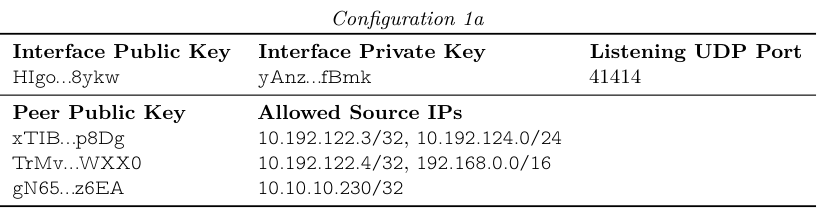
\includegraphics[width=0.92\linewidth,height=0.7\textheight,keepaspectratio]{src/images/Pasted_image_20261001214515.png}
  \caption{Pasted Image 20261001214515}
  \label{fig:Pasted_image_20261001214515}
\end{figure}

Decide quali coppie \((\text{Peer Public Key, Allowed Source IP})\)
possono instradare nell'interfaccia wireguard.

Opzionalmente e' possibile specificare verso quale endpoint inoltrare il
pacchetto. L'\textbf{endpoint} identifica l'indirizzo ip e la porta UDP
su cui il demone WireGuard e' in ascolto.

Brevemente il flusso dei dati e' il seguente:

\begin{itemize}
\tightlist
\item
  l'interfaccia \passthrough{\lstinline!wg0!} riceve un pacchetto
\item
  il client incapsula il pacchetto all'interno di una datagramma UPD il
  cui payload viene crittografato utilizzando
  \passthrough{\lstinline!ChaCha20Poly1305!}
\item
  il client invia il datagramma all'endpoint specificato, oppure
  imparato dal Wireguard in precedenza.
\item
  il server riceve il dataramma, verifica la correttezza nella
  \emph{cryptokey routing table}
\item
  il server autentica e decripta il messaggio ed estrae il pacchetto
  originario
\item
  il pacchetto originario viene inserito in una coda nell'interfaccia
  \(\text{wg}0\)
\end{itemize}
